\documentclass{beamer}
\usepackage{graphicx}
\usepackage{amsmath}
\usepackage{tikz}
\usepackage{amssymb}
\usepackage{hyperref}
\usepackage{booktabs}
\usepackage{multicol}
\usetikzlibrary{arrows.meta, positioning, shapes.geometric}

\title{Multi-Robot Path Optimization for Search and Rescue}
\author{Team 14}
\institute{German University in Cairo}
\date{\today}

\begin{document}

\begin{frame}
    \titlepage
\end{frame}

\begin{frame}{Outline}
    \tableofcontents
\end{frame}

\section{Problem Overview}

\begin{frame}{Problem Overview}
    \begin{columns}
        \begin{column}{0.6\textwidth}
            \textbf{Objective:} Optimize paths for multiple robots to explore an unknown area.
            \vspace{1cm}
            
            \textbf{Key Challenges:}
            \begin{itemize}
                \item Maximize area coverage.
                \item Maintain communication between robots.
                \item Adhere to energy (battery) limitations.
                \item Avoid obstacles and collisions.
                \item Handle network disconnections gracefully.
            \end{itemize}
        \end{column}
        \begin{column}{0.4\textwidth}
            \begin{figure}
                \centering
                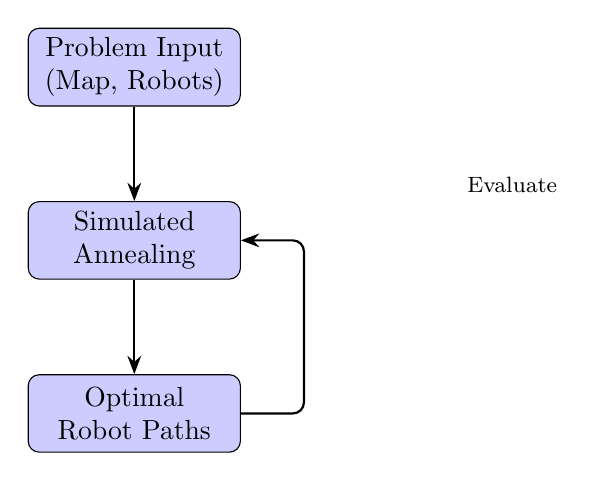
\begin{tikzpicture}[
                    node distance=1.2cm,
                    block/.style={rectangle, draw, fill=blue!20, text width=7em, text centered, rounded corners, minimum height=2.8em},
                    arrow/.style={-Stealth, thick}
                ]
                \node[block] (input) {Problem Input (Map, Robots)};
                \node[block, below=of input] (sa) {Simulated Annealing};
                \node[block, below=of sa] (output) {Optimal Robot Paths};
                
                \draw[arrow] (input) -- (sa);
                \draw[arrow] (sa) -- (output);
                \draw[arrow, rounded corners] (output.east) -- ++(0.8,0) |- (sa.east);
                \node[font=\footnotesize, align=center] at (4.8, -1.5) {Evaluate};
                \end{tikzpicture}
                \caption{High-level overview of the optimization process.}
            \end{figure}
        \end{column}
    \end{columns}
\end{frame}

\section{Assumptions}


\begin{frame}{Assumptions at a Glance}
    \begin{columns}
        \begin{column}{0.5\textwidth}
            \begin{itemize}
                \item \textbf{Environment:} Discrete grid map with unexplored cells, free space, and obstacles.
                \item \textbf{Robots:} Team of identical robots.
                \item \textbf{Obstacles:} Unknown initially, discovered during exploration.
                \item \textbf{Motion:} Discrete time steps, 4-connected grid (up, down, left, right, stay).
                \item \textbf{Energy:} Finite budget limits travel distance.
                \item \textbf{Communication:} Position sharing; link quality degrades with distance.
            \end{itemize}
        \end{column}
        \begin{column}{0.5\textwidth}
            \begin{center}
            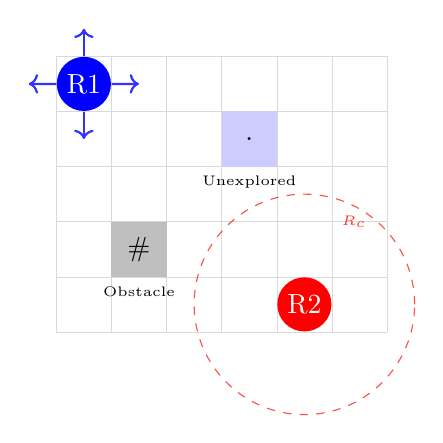
\begin{tikzpicture}[scale=0.7]
                % Grid
                \draw[step=1cm, color=gray!30, very thin] (0,0) grid (6,5);
                
                % Cells
                \fill[gray!50] (1,1) rectangle (2,2);
                \node at (1.5,1.5) {\#};
                \node[below, font=\tiny] at (1.5,1) {Obstacle};

                \fill[blue!20] (3,3) rectangle (4,4);
                \node at (3.5,3.5) {.};
                \node[below, font=\tiny] at (3.5,3) {Unexplored};

                % Robots
                \node[circle, fill=blue, text=white, inner sep=2pt] (r1) at (0.5, 4.5) {R1};
                \node[circle, fill=red, text=white, inner sep=2pt] (r2) at (4.5, 0.5) {R2};
                
                % Communication Radius
                \draw[dashed, red!70] (r2) circle (2cm);
                \node[red!80, font=\tiny, right] at (5, 2) {$R_c$};
                
                % Motion
                \draw[->, thick, blue!80] (r1) -- ++(1,0);
                \draw[->, thick, blue!80] (r1) -- ++(-1,0);
                \draw[->, thick, blue!80] (r1) -- ++(0,1);
                \draw[->, thick, blue!80] (r1) -- ++(0,-1);
            \end{tikzpicture}
            \end{center}
        \end{column}
    \end{columns}
\end{frame}

\section{Solution Representation}

\begin{frame}{How a Solution Looks Like}
    A solution is a set of paths, one for each robot, over a fixed time horizon $K$.
    
    \vspace{0.3cm}
    \textbf{Path Array:} A 3D array $path\_array[r][t] = (x, y)$ stores the position of robot $r$ at time step $t$.
    
    \begin{center}
    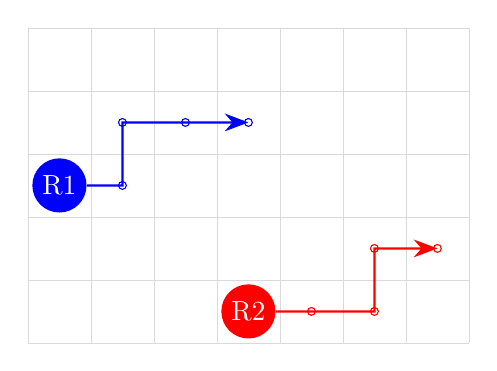
\begin{tikzpicture}[scale=0.8]
        % Grid
        \draw[step=1cm, color=gray!30, very thin] (0,0) grid (7,5);
        
        % Robot 1
        \node[circle, fill=blue, text=white, inner sep=2pt] (r1_0) at (0.5, 2.5) {R1};
        \draw[blue, thick, -{Stealth[length=3mm]}] (r1_0) -- (1.5, 2.5) -- (1.5, 3.5) -- (2.5, 3.5) -- (3.5, 3.5);
        \node[draw, circle, blue, inner sep=1pt] at (1.5, 2.5) {};
        \node[draw, circle, blue, inner sep=1pt] at (1.5, 3.5) {};
        \node[draw, circle, blue, inner sep=1pt] at (2.5, 3.5) {};
        \node[draw, circle, blue, inner sep=1pt] at (3.5, 3.5) {};

        % Robot 2
        \node[circle, fill=red, text=white, inner sep=2pt] (r2_0) at (3.5, 0.5) {R2};
        \draw[red, thick, -{Stealth[length=3mm]}] (r2_0) -- (4.5, 0.5) -- (5.5, 0.5) -- (5.5, 1.5) -- (6.5, 1.5);
        \node[draw, circle, red, inner sep=1pt] at (4.5, 0.5) {};
        \node[draw, circle, red, inner sep=1pt] at (5.5, 0.5) {};
        \node[draw, circle, red, inner sep=1pt] at (5.5, 1.5) {};
        \node[draw, circle, red, inner sep=1pt] at (6.5, 1.5) {};
    \end{tikzpicture}
    
    \vspace{0.5cm}
    \centering
    Example paths for 2 robots over 4 time steps.
    \end{center}
\end{frame}

\section{The Objective Function}

\begin{frame}{Objective Function: The Goal}
The goal is to \textbf{maximize} a composite objective function that balances multiple competing goals:
\vspace{0.5cm}
\begin{align*}
    f = \quad & \alpha \cdot \text{Coverage} \\
              & + \beta \cdot \text{Connectivity} \\
              & - \gamma \cdot \text{Disconnection Penalty}
\end{align*}
\vspace{0.5cm}
where $\alpha, \beta, \gamma$ are weights to tune the importance of each component.
\end{frame}

\begin{frame}{Objective 1: Coverage}
    \textbf{Goal:} Maximize the number of unique unexplored cells visited by all robots.
    \[ \text{Coverage} = \sum_{\text{all cells (x,y)}} C_{x,y} \]
    where $C_{x,y}=1$ if a cell $(x,y)$ is visited, and 0 otherwise.
    
    \begin{center}
    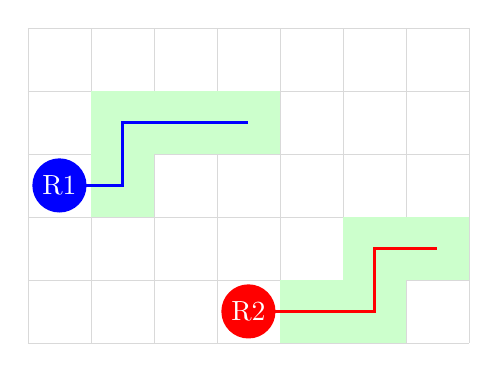
\begin{tikzpicture}[scale=0.8]
        % Grid
        \draw[step=1cm, color=gray!30, very thin] (0,0) grid (7,5);
        
        % Visited cells
        \fill[green!20] (1,2) rectangle (2,3);
        \fill[green!20] (1,3) rectangle (2,4);
        \fill[green!20] (2,3) rectangle (3,4);
        \fill[green!20] (3,3) rectangle (4,4);
        \fill[green!20] (4,0) rectangle (5,1);
        \fill[green!20] (5,0) rectangle (6,1);
        \fill[green!20] (5,1) rectangle (6,2);
        \fill[green!20] (6,1) rectangle (7,2);

        % Robot paths
        \draw[blue, thick] (0.5, 2.5) -- (1.5, 2.5) -- (1.5, 3.5) -- (2.5, 3.5) -- (3.5, 3.5);
        \draw[red, thick] (3.5, 0.5) -- (4.5, 0.5) -- (5.5, 0.5) -- (5.5, 1.5) -- (6.5, 1.5);
        
        \node[circle, fill=blue, text=white, inner sep=2pt] at (0.5, 2.5) {R1};
        \node[circle, fill=red, text=white, inner sep=2pt] at (3.5, 0.5) {R2};
    \end{tikzpicture}
    
    \vspace{0.5cm}
    \centering
    Shaded cells are newly explored and contribute to the coverage score.
    \end{center}
\end{frame}

\begin{frame}{Objective 2: Connectivity}
    \textbf{Goal:} Encourage robots to stay close to each other to ensure reliable communication.
    \[ \text{Connectivity} = \sum_{t=0}^{K} \sum_{i<j} W_{ij,t} \]
    The link quality $W_{ij,t}$ between robots $i$ and $j$ is higher when they are closer:
    \[ W_{ij,t} = \frac{1}{1+d_{ij,t}} \quad (\text{if } d_{ij,t} \le R_c) \]
    
    \begin{center}
    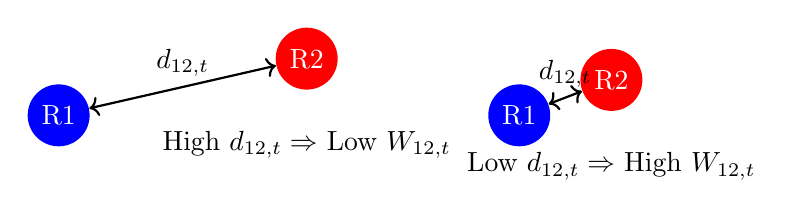
\begin{tikzpicture}[scale=0.9]
        \node[circle, fill=blue, text=white, inner sep=3pt] (r1) at (0,0) {R1};
        \node[circle, fill=red, text=white, inner sep=3pt] (r2) at (3.5,0.8) {R2};
        
        \draw[<->, thick] (r1) -- (r2) node[midway, above] {$d_{12,t}$};
        \node[below=0.4cm of r2, align=center] {High $d_{12,t} \Rightarrow$ Low $W_{12,t}$};
        
        \node[circle, fill=blue, text=white, inner sep=3pt] (r3) at (6.5,0) {R1};
        \node[circle, fill=red, text=white, inner sep=3pt] (r4) at (7.8,0.5) {R2};
        
        \draw[<->, thick] (r3) -- (r4) node[midway, above] {$d_{12,t}$};
        \node[below=0.4cm of r4, align=center] {Low $d_{12,t} \Rightarrow$ High $W_{12,t}$};
    \end{tikzpicture}
    \end{center}
\end{frame}

\begin{frame}{Penalty: Disconnection}
    \textbf{Goal:} Penalize robots that become disconnected from the main communication network.
    \[ P_{\text{disconnect}} = \sum_{t=0}^{K} \sum_{i=1}^{N} \delta_{i,t} \cdot d_{i,\text{net},t} \]
    \begin{itemize}
        \item $\delta_{i,t}=1$ if robot $i$ is disconnected at time $t$.
        \item $d_{i,\text{net},t}$ is the distance from the disconnected robot to the closest robot in the main network.
    \end{itemize}
    
    \begin{center}
    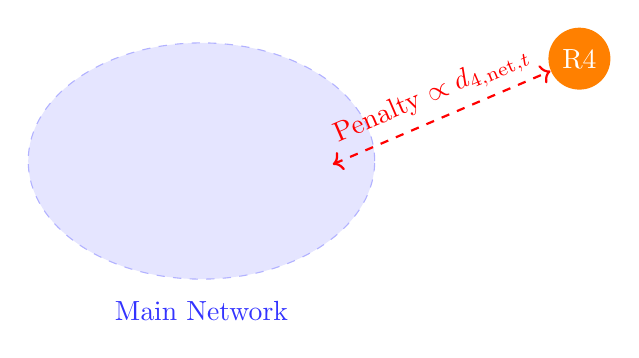
\begin{tikzpicture}
        % Main network
        \node[circle, fill=blue, text=white, inner sep=3pt] (r1) at (0,0) {R1};
        \node[circle, fill=red, text=white, inner sep=3pt] (r2) at (1,1.5) {R2};
        \node[circle, fill=green!60!black, text=white, inner sep=3pt] (r3) at (2.5,0.5) {R3};
        \draw[thick, blue!50] (r1) -- (r2);
        \draw[thick, blue!50] (r2) -- (r3);
        \draw[thick, blue!50] (r1) -- (r3);
        \draw[dashed, blue!30, fill=blue!10] (1.2, 0.7) ellipse (2.2cm and 1.5cm);
        \node[blue!80] at (1.2, -1.2) {Main Network};

        % Disconnected robot
        \node[circle, fill=orange, text=white, inner sep=3pt] (r4) at (6, 2) {R4};
        
        % Penalty line
        \draw[<->, thick, red, dashed] (r3) -- (r4) node[midway, above, sloped] {Penalty $\propto d_{4,\text{net},t}$};
    \end{tikzpicture}
    \end{center}
\end{frame}


\section{Constraints}

\begin{frame}{Hard Constraints (Feasibility)}
A path is only valid if it satisfies all hard constraints. An infeasible path is given a very poor score (e.g., -1).

\begin{multicols}{2}
    \textbf{1. Map Bounds:}
    Robots must stay within the grid.
    \[ 0 \le x_{i,t} < N, \quad 0 \le y_{i,t} < M \]
    
    \textbf{2. Motion Model:}
    Robots can only move to adjacent cells (4-way) or stay put.
    \[ |x_{i,t}-x_{i,t-1}| + |y_{i,t}-y_{i,t-1}| \le 1 \]
    
    \textbf{3. Energy Budget:}
    Total distance traveled cannot exceed the battery limit $\ell$.
    \[ \sum_{\tau=1}^{t} \text{dist}(p_{i,\tau}, p_{i,\tau-1}) \le \ell \]
    
    \columnbreak
    
    \textbf{4. Obstacle Avoidance:}
    Robots cannot occupy cells with known obstacles.
    \[ p_{i,t} \notin \text{Obstacles} \]
    
    \textbf{5. Collision Avoidance:}
    No two robots can be in the same cell at the same time.
    \[ p_{i,t} \neq p_{j,t} \quad \forall i \neq j \]
\end{multicols}
\end{frame}



\section{Simulation Video}

\begin{frame}{Live Simulation Demo}

\end{frame}

\end{document}
